\begin{minipage}[t]{100mm}
\vspace{3mm}

\section*{Parringsritual -- Mumier}


\section*{Dagens sang}
\begin{center}
Vi bynne å vi stajsfolk

vi sønge om vå skønne ø;

en kigge øv’e marke,

å øv’e skov å sø.

E blombej det æ fyldt med blomme,

å olt æ ve å ve’ så grønt.

Vi gleje vås te’e somme.

vo olting æ så køhnt.

Vå ø æ som en kal’gå

mæ blomme o væt efeltre,

vo olting æ så dejle,

ven langs e strand’ en ge.

Vi juble – der æ it dæ tynge,

å tej væranne om e hals.

Vi sammel ge’ å synge

som e bølle om våt Als.

Et sproch, som ingen anne,

så køhnt – å mæ så fin en klang;

å olti’ æ vi manne

som seje det mæ sang;

e faul di sønge olti’ om e,

e svane bøje fint e hals,

å ingen stej i verden

e sang æ som o Als.
\end{center}

\section*{Dagens sætning - Pizza Sætningen}
Hvis en rund pizza bliver delt i $8, 12, 16, \dots$ slices ved fra et vilkårligt punkt på pizzaen at inddele den i slices med samme vinkel, så vil man hvis man spiser hvert andet stykke rundt, have spist halvdelen af pizzaen.
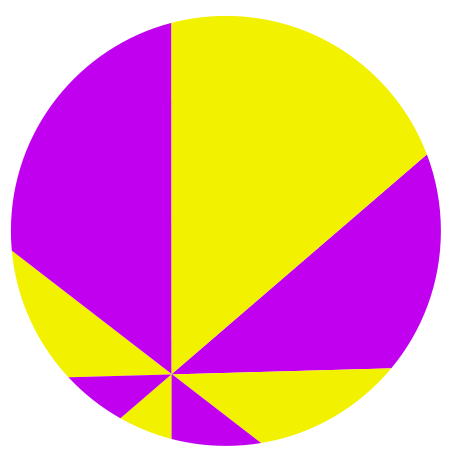
\includegraphics[width=\textwidth]{Pizzathm.png}
\end{minipage}
